% !TEX TS-program = XeLaTeX
% use the following command:
% all document files must be coded in UTF-8
\documentclass[spanish]{textolivre}
% build HTML with: make4ht -e build.lua -c textolivre.cfg -x -u article "fn-in,svg,pic-align"

\journalname{Texto Livre}
\thevolume{15}
%\thenumber{1} % old template
\theyear{2022}
\receiveddate{\DTMdisplaydate{2022}{10}{31}{-1}} % YYYY MM DD
\accepteddate{\DTMdisplaydate{2022}{11}{4}{-1}}
\publisheddate{\DTMdisplaydate{2022}{11}{18}{-1}}
\corrauthor{Pilar Ibáñez-Cubillas}
\articledoi{10.35699/1983-3652.2022.41617}
%\articleid{NNNN} % if the article ID is not the last 5 numbers of its DOI, provide it using \articleid{} commmand 
% list of available sesscions in the journal: articles, dossier, reports, essays, reviews, interviews, editorial
\articlesessionname{dossier}
\runningauthor{Ibáñez-Cubillas} 
%\editorname{Leonardo Araújo} % old template
\sectioneditorname{Daniervelin Pereira}
\layouteditorname{Leonado Araújo}

\title{Factores neurodidácticos de la enseñanza basada en TIC: aportes para la formación docente}
\othertitle{Fatores neurodidáticos no ensino baseado nas TIC: contribuições para a formação de professores}
\othertitle{Neurodidactic factors in ICT-based teaching: contributions to teacher education}
% if there is a third language title, add here:
%\othertitle{Artikelvorlage zur Einreichung beim Texto Livre Journal}

\author[1]{Pilar Ibáñez-Cubillas~\orcid{0000-0001-7117-5746}\thanks{Email: \href{mailto:pcubillas@uma.es}{pcubillas@uma.es}}}
\affil[1]{Universidad de Málaga, Facultad de Ciencias de la Educación, Departamento de Didáctica y Organización Escolar, Málaga, España.}

\addbibresource{article.bib}
% use biber instead of bibtex
% $ biber article

% used to create dummy text for the template file
\definecolor{dark-gray}{gray}{0.35} % color used to display dummy texts
\usepackage{lipsum}
\SetLipsumParListSurrounders{\colorlet{oldcolor}{.}\color{dark-gray}}{\color{oldcolor}}

% used here only to provide the XeLaTeX and BibTeX logos
\usepackage{hologo}

% if you use multirows in a table, include the multirow package
\usepackage{multirow}

% provides sidewaysfigure environment
\usepackage{rotating}

% CUSTOM EPIGRAPH - BEGIN 
%%% https://tex.stackexchange.com/questions/193178/specific-epigraph-style
\usepackage{epigraph}
\renewcommand\textflush{flushright}
\makeatletter
\newlength\epitextskip
\pretocmd{\@epitext}{\em}{}{}
\apptocmd{\@epitext}{\em}{}{}
\patchcmd{\epigraph}{\@epitext{#1}\\}{\@epitext{#1}\\[\epitextskip]}{}{}
\makeatother
\setlength\epigraphrule{0pt}
\setlength\epitextskip{0.5ex}
\setlength\epigraphwidth{.7\textwidth}
% CUSTOM EPIGRAPH - END

% LANGUAGE - BEGIN
% ARABIC
% for languages that use special fonts, you must provide the typeface that will be used
% \setotherlanguage{arabic}
% \newfontfamily\arabicfont[Script=Arabic]{Amiri}
% \newfontfamily\arabicfontsf[Script=Arabic]{Amiri}
% \newfontfamily\arabicfonttt[Script=Arabic]{Amiri}
%
% in the article, to add arabic text use: \textlang{arabic}{ ... }
%
% RUSSIAN
% for russian text we also need to define fonts with support for Cyrillic script
% \usepackage{fontspec}
% \setotherlanguage{russian}
% \newfontfamily\cyrillicfont{Times New Roman}
% \newfontfamily\cyrillicfontsf{Times New Roman}[Script=Cyrillic]
% \newfontfamily\cyrillicfonttt{Times New Roman}[Script=Cyrillic]
%
% in the text use \begin{russian} ... \end{russian}
% LANGUAGE - END

% EMOJIS - BEGIN
% to use emoticons in your manuscript
% https://stackoverflow.com/questions/190145/how-to-insert-emoticons-in-latex/57076064
% using font Symbola, which has full support
% the font may be downloaded at:
% https://dn-works.com/ufas/
% add to preamble:
% \newfontfamily\Symbola{Symbola}
% in the text use:
% {\Symbola }
% EMOJIS - END

% LABEL REFERENCE TO DESCRIPTIVE LIST - BEGIN
% reference itens in a descriptive list using their labels instead of numbers
% insert the code below in the preambule:
%\makeatletter
%\let\orgdescriptionlabel\descriptionlabel
%\renewcommand*{\descriptionlabel}[1]{%
%  \let\orglabel\label
%  \let\label\@gobble
%  \phantomsection
%  \edef\@currentlabel{#1\unskip}%
%  \let\label\orglabel
%  \orgdescriptionlabel{#1}%
%}
%\makeatother
%
% in your document, use as illustraded here:
%\begin{description}
%  \item[first\label{itm1}] this is only an example;
%  % ...  add more items
%\end{description}
% LABEL REFERENCE TO DESCRIPTIVE LIST - END


% add line numbers for submission
%\usepackage{lineno}
%\linenumbers

\begin{document}
\maketitle

\begin{polyabstract}
\begin{abstract}
Cambiar del paradigma centrado en la enseñanza al centrado en el aprendizaje, implica mejorar la formación inicial docente para que los factores neurodidácticos de la transformación escolar se optimicen y, se integren adecuadamente las Tecnologías de la Información y la Comunicación (TIC) en los espacios educativos. Teniendo en cuenta las dificultades que enfrentan los docentes ante el uso estrictamente didáctico de las TIC, el presente documento alude a las aportaciones de la neurodidáctica y a las exigencias de las TIC para la actualización de la formación inicial docente. A grandes rasgos, se aboga por la incorporación del contenido de las neurociencias en los currículos de la formación docente para que deriven en intervenciones didácticas eficientes que fomenten el aprendizaje significativo, así como, el desarrollo cerebral y psicodinámico. Por otro lado, se aboga por la formación docente a partir de modelos que orientan la integración efectiva de las TIC en el aula, como pueden ser el modelo TPACK, el modelo SAMR; el modelo revisado de BLOOM o el modelo de Maslow-Gerstein, lo que lleva a considerar los factores neurodidácticos que inciden en la enseñanza virtual y su repercusión en la persistencia, el éxito y el aprovechamiento académico.

\keywords{Formación docente \sep Modelos de integración didáctica \sep Neurodidáctica \sep TIC}
\end{abstract}

\begin{portuguese}
\begin{abstract}
Passar de um paradigma centrado no ensino para um paradigma centrado na aprendizagem implica melhorar a formação inicial de professores de modo a otimizar os fatores neurodidáticos da transformação escolar e a integrar devidamente as Tecnologias de Informação e Comunicação (TIC) nos espaços educativos. Tendo em vista as dificuldades enfrentadas pelos professores no uso estritamente didático das TIC, este documento refere-se às contribuições da neurodidática e às exigências das TIC para a atualização da formação inicial de professores. Em termos gerais, defende a incorporação de conteúdos neurocientíficos nos currículos de formação de professores para levar a intervenções didáticas eficientes que promovam uma aprendizagem significativa, bem como o desenvolvimento cerebral e psicodinâmico. Por outro lado, a formação de professores é defendida com base em modelos que orientam a integração efetiva das TIC na sala de aula, tais como o modelo TPACK, o modelo SAMR, o modelo BLOOM revisto ou o modelo Maslow-Gerstein, o que leva a considerar os fatores neurodidáticos que incidem no ensino virtual e o seu impacto na persistência, sucesso e realização acadêmica.

\keywords{Formação de professores \sep Modelos de integração educacional \sep Neurodidática \sep TIC}
\end{abstract}
\end{portuguese}

\begin{english}
\begin{abstract}
Shifting from a teaching-centred to a learning-centred paradigm implies improving initial teacher training so that the neurodidactic factors of school transformation are optimised and Information and Communication Technologies (ICT) are properly integrated into educational spaces. Considering the difficulties faced by teachers in the strictly didactic use of ICT, this document refers to the contributions of neurodidactics and the demands of ICT for the updating of initial teacher training. Broadly speaking, it argues for the incorporation of neuroscience content in teacher education curricula to lead to efficient didactic interventions that promote meaningful learning, as well as brain and psychodynamic development. On the other hand, teacher training is advocated on the basis of models that guide the effective integration of ICT in the classroom, such as the TPACK model, the SAMR model, the revised BLOOM model or the Maslow-Gerstein model, which leads to consider the neurodidactic factors that concern virtual teaching and its impact on persistence, success and academic achievement.

\keywords{Teacher education \sep Educational integration models \sep Neurodidactics \sep ICT}
\end{abstract}
\end{english}
% if there is another abstract, insert it here using the same scheme
\end{polyabstract}

\section{La neurodidáctica en la formación inicial docente}\label{sec-intro}
Es indudable que la transformación curricular, organizativa y metodológica que está ocurriendo en las aulas, no solo afecta a aspectos formales y externos de la relación entre alumnado y docente, sino que, sobre todo afecta a factores internos ligados a la efectividad del aprendizaje, como son los neuropedagógicos que se implican en la relación didáctica.

El vuelco que han dado las aulas, en todos los niveles y en todos los lugares con la incorporación e integración de las Tecnologías de la Información y la Comunicación (TIC) como soporte de esa relación didáctica, merece un aporte desde la perspectiva de cómo mejorar la formación inicial docente para que los factores neurodidácticos de la transformación escolar se optimicen.

Entendemos que las fuentes para la actualización de la formación inicial docente desde las nuevas exigencias de las TIC y la neurociencia son las siguientes:

\begin{enumerate}
    \item La extensión y modernización de las funciones y competencias docentes. Para \textcite{schimf-herken_modelo_2006}, las nuevas necesidades sociales llevan aparejadas nuevas estrategias y formas de escolarización que amplían, extienden y actualizan las exigencias sociales al profesorado y ponen de relieve la oportunidad de transformación de la formación docente para atender esas nuevas competencias que la sociedad demanda. La educación inclusiva, la educación con TIC, la educación emocional y la neuroeducación, están dentro de esas nuevas competencias que hoy se exigen. 
    \item El contenido de la neurociencia debe ser incorporado a los currículos de la formación docente. \textcite{calzadilla_perez_integracion_2017} señala que, al menos, el contenido de la formación inicial docente debería considerar el estudio de la fisiología del cerebro, funcionamiento y desarrollo; la funcionalidad y plasticidad cerebral; las bases neurológicas del desarrollo psicomotor; el sistema nervioso y sistemas sensoriales; las funciones ejecutivas; las bases neurofisiológicas del desarrollo del pensamiento en edad escolar; el vínculo del pensamiento con otras funciones psíquicas superiores; los sistemas sensorio motores y el desarrollo del aprendizaje y; los daños al sistema nervioso central y efectos en el aprendizaje.
    \item La transferencia a la educación de profesionales de la formación de las metodologías exitosas en la enseñanza no universitaria. Revindicando el principio de isomorfismo, por el que un docente debería ser formado con las mismas metodologías participativas e innovadoras que debe aprender para aplicar en el futuro, \textcite{arturo_obando_plan_2020} señala que la formación docente debería realizarse con la gestión emocional que va asociada al aprendizaje, con la activación y estimulación  de las destrezas neurocognitivas, con atención especial al desarrollo del cerebro del futuro docente, activando la curiosidad y proponiendo desafíos de aprendizaje, potenciando los talentos individuales, usando la creatividad, apoyándose en la variabilidad personal y el uso de diferentes estilos de aprendizaje, enfatizando el espíritu emprendedor que facilita en el aprendiz el control del  miedo al fracaso y, evidentemente, con la incorporación de las últimas y más variadas tecnologías al servicio del aprendizaje.
    \item La aplicación de los resultados de la investigación en neurociencia es revisada por \textcite{acta_caraballo_concepcion_2021} para proponer que en las aulas de formación inicial docente se difundan los resultados de los estudios sobre los factores neurodidácticos que determinan el aprendizaje en las distintas etapas de la educación.
\end{enumerate}

La oportunidad de modificación normativa de los currículos formativos es algo que hay que aprovechar para incluir cambios de esta naturaleza en varios niveles: proponiendo contenidos complementarios, incluyendo materias específicas sobre neurodidáctica en los currículos formativos o, incluso, proponiendo innovaciones institucionales para modificar e intensificar las estrategias que propician la enseñanza basada en TIC y en los avances de la neurodidáctica.

\section{La formación docente para la integración de las TIC en el aula}\label{sec-normas}
Las principales barreras, ampliamente estudiadas \cite{bingimlas_barriers_2009}, para la implementación de la tecnología en las aulas, son las referidas a las barreras intrínsecas, es decir, aquellas que están directamente asociadas con el docente; como la falta de preparación, la resistencia al cambio y, especialmente, la falta de confianza en el uso de la tecnología. La investigación científica nacional e internacional en el campo de la tecnología educativa es unánime al afirmar que el elemento clave de los procesos de integración tecnológica en los entornos escolares es el profesor. La integración de la tecnología en un contexto educativo requiere que los docentes reciban la formación adecuada y comprendan el potencial de la tecnología para sus prácticas. Siempre que ha faltado una labor estratégica de formación docente, sobre todo a través de la formación continua, el resultado ha sido el uso marginal de equipos, \textit{software} o plataformas adquiridos o el mantenimiento de prácticas docentes tradicionales sin ningún tipo de innovación (por ejemplo, el uso de una pizarra interactiva para proyectar diapositivas).

Hay que tener en cuenta que las tecnologías educativas tradicionales (proyectores, vídeo...) han evolucionado a una velocidad vertiginosa, dando como resultado tecnologías digitales (ordenadores, portátiles, dispositivos móviles, tabletas, \textit{smartphones}, aplicaciones de interacción educativa, \textit{software} de simulación, \textit{software} en 3D, \textit{software} colaborativo, etc.) cada vez más completas en sus potencialidades y efímeras en su originalidad o innovación. La enseñanza con medios audiovisuales, en particular con las tecnologías en su vertiente 2.0 (web social) es, por tanto, un reto para la sociedad y para los docentes en particular, que aún tienen muchas dificultades para utilizar estas herramientas en su dimensión pedagógica entendida como potencial de inclusión en el aula.

Por tanto, es urgente reflexionar sobre cómo la formación del profesorado puede facilitar los procesos de integración de las TIC, mediante el reconocimiento del valor pedagógico de las herramientas tecnológicas y el desarrollo de las competencias digitales necesarias para su uso. En este sentido, recientemente hemos revisado los modelos alternativos que la integración de las TIC puede presentar en las aulas: (a) modelo TPACK; (b) modelo SAMR; (c) modelo revisado de BLOOM; y (d) modelo de Maslow-Gerstein.

\subsection{Modelo TPACK}\label{sec-conduta}
El docente necesita entender que la tecnología no es neutral, es decir, cada recurso tecnológico ofrece oportunidades y limitaciones, por lo que deja al docente la tarea de hacerla más adecuada a través de una propuesta didáctica consolidada y adaptada al contenido, al contexto, a los destinatarios y al objetivo de aprendizaje \cite{koehler_what_2009}.

El modelo TPACK (originalmente TPCK) se basa en tres elementos principales para el conocimiento de los docentes: contenido, pedagogía y tecnología, y tiene como objetivo ayudarles a comprender que la tecnología educativa y el conocimiento pedagógico del contenido deben interactuar para contribuir a una enseñanza eficaz con tecnología. Es la interacción entre el Conocimiento Tecnológico, el Conocimiento Pedagógico y el Conocimiento del Contenido lo que genera otros cuerpos de conocimiento representados como PCK (conocimiento pedagógico del contenido), TCK (conocimiento tecnológico del contenido), TPK (conocimiento tecnológico pedagógico) y TPACK (conocimiento pedagógico del contenido tecnológico) \cite{Koehle_2014}. 

PCK: el “conocimiento pedagógico del contenido” se sustenta en la idea de conocimiento pedagógico de \textcite{shulman_knowledge_1987}, que defiende este tipo de conocimiento como un medio para reformar y profesionalizar la enseñanza. Cuando el modelo PCK es desarrollado y adquirido por el docente, se desencadena esta transformación y, por tanto, el docente debe ser capaz de interpretar el contenido y de representarlo de diversas formas, adecuar los conocimientos al alumnado y también debe ser capaz de adaptarse al contexto. Por tanto, este conocimiento abarca las principales actividades docentes, como el aprendizaje, el currículo o la evaluación, de lo que se concluye que el conocimiento de estas áreas, las conexiones entre ellas y la reflexión de estas por parte de los docentes son fundamentales para una enseñanza eficaz.

TCK: el “conocimiento tecnológico del contenido” es el punto de convergencia entre tecnología y contenido. Los docentes no solo tienen que dominar los contenidos enseñados, sino que también deben ser conscientes de que una determinada experiencia de aprendizaje puede cambiar dependiendo de la tecnología utilizada, por lo tanto, deben entender que ciertas tecnologías son más adecuadas para desarrollar aprendizajes específicos; y que una selección inapropiada puede producir cambios en la comprensión del contenido, o que un determinado contenido puede influir en el uso de la tecnología cambiando su función principal / inicial. El desarrollo de recursos tecnológicos adecuados para fines educativos específicos está directamente ligado a la comprensión del impacto de la tecnología en la práctica y el contenido requiere una correcta selección de la tecnología, determinando el tipo de contenido que se puede enseñar y viceversa. Es decir, el contenido define el tipo de tecnología que se puede utilizar.

TPK: “conocimiento tecnológico pedagógico” implica comprender cómo el proceso de enseñanza y aprendizaje puede cambiar en función de la herramienta tecnológica seleccionada. Se trata de conocer las posibilidades y limitaciones de un amplio abanico de recursos tecnológicos educativos y su relación con los materiales, para desarrollar estrategias de enseñanza en función de las necesidades. Por tanto, TPK requiere de mentes abiertas y buscar aplicaciones alternativas del uso de la tecnología, como de blogs o podcasts en la calidad de recursos didácticos, siendo el objetivo inicial de estas herramientas la comunicación o el entretenimiento. Así, los docentes necesitan desarrollar habilidades que les permitan ir más allá de los usos comunes de las tecnologías y, por tanto, reconfigurar la finalidad de estos recursos con un matiz pedagógico personalizado.

TPACK: el “conocimiento tecnológico pedagógico de los contenidos” es el resultado de la interacción de los diferentes modelos. Con este modelo, la enseñanza es significativa, eficaz y hábil en el uso de la tecnología. \textcite{koehler_what_2009} con TPACK pretendían resaltar que los docentes deben interpretar los tres componentes básicos (contenido, pedagogía y tecnología) en su conjunto, ya que es en la relación entre ellos donde el docente puede desarrollar una enseñanza eficaz en la que se promueva una flexibilidad  cognitiva de los profesionales y unas habilidades para resolver problemas educativos, recordando que el uso de la tecnología con fines pedagógicos es un equilibrio dinámico entre todos los componentes.

\subsection{Modelo SAMR}\label{sec-fmt-manuscrito}
Tal y como indican \textcite{garcia-utrera_modelo_2014} el modelo SAMR (de las siglas en inglés, \textit{Substitution, Augmentation, Modification, Redefinition}) fue desarrollado por el Dr. Ruben D. Puentedura, aunque la primera versión oficial fue desarrollada y aprobada por un grupo de expertos del Estado de Maine en Estados Unidos.

El modelo SAMR tiene como finalidad ayudar a los docentes a evaluar la forma en que están incorporando las tecnologías en sus aulas y de esta manera, conocer qué tipo de usos de la tecnología tienen un mayor o menor efecto sobre el aprendizaje de los estudiantes \cite{puentedura_models_2008}. Consiste en un conjunto jerárquico de dos capas (mejora y transformación) y cuatro niveles (correspondientes a las siglas del modelo) que describen el uso de herramientas tecnológicas \cite{garcia-utrera_modelo_2014} y sirven para la mejora y la transformación. 

En cuanto a la mejora, la \textit{sustitución} es el nivel más bajo de uso de la tecnología. Se sustituye una herramienta por otra sin que exista un cambio metodológico, por ejemplo, en vez de usar papel y lápiz se escribe en un procesador de texto, sin hacer uso alguno de sus demás funciones. Por su parte, el \textit{aumento}, indica que la tecnología remplaza otra herramienta y le añade mejoras funcionales que facilitan la tarea; sin embargo, no hay un cambio en la metodología y el efecto en los resultados de aprendizaje de los estudiantes puede ser mínimo o nulo. Por ejemplo, usar el corrector ortográfico o las funciones de copiar-pegar en el procesador de texto.

En cuanto a la transformación, exige \textit{modificación} o cambio metodológico en el cual la tarea a realizar es rediseñada por la introducción de la tecnología. En el ejemplo citado anteriormente, el procesador de texto permite ver mejoras significativas en el desempeño académico de los estudiantes si se incorporan herramientas en red como el correo electrónico, los blogs y las redes sociales. O, más allá de lo anterior, \textit{redefinición}. En este último nivel se crean nuevas actividades y ambientes de aprendizaje que, sin el uso de la tecnología disponible, serían imposibles. Por ejemplo, el alumnado colabora en tiempo real en un mismo documento y añaden a su producto final elementos multimedia creados por ellos mismos.


\subsection{Modelo revisado de Bloom para la era digital}\label{sec-formato}
La taxonomía de Bloom y la taxonomía revisada de Bloom para la era digital son herramientas clave para los docentes y los encargados del diseño de capacitaciones. Benjamín Bloom publicó la taxonomía original en los años de 1950 y Lorin Anderson y Krathwohl le hicieron revisiones en el 2000. Pero desde la más reciente publicación de la taxonomía han ocurrido muchos cambios y desarrollos que deben tenerse en cuenta.

En el año de 1956, Benjamín Bloom desarrolló su taxonomía de Objetivos Educativos. Dicha taxonomía se convirtió en herramienta clave para estructurar y comprender el proceso de aprendizaje. De los tres dominios que comprende el aprendizaje, se centró en el Cognitivo. Los tres dominios son: el Cognitivo (procesar información, conocimiento y habilidades mentales), el Afectivo (actitudes y sentimientos), el Psicomotor (habilidades manipulativas, manuales o físicas). 

La propuesta es un continuo que parte de Habilidades de Pensamiento de Orden Inferior (LOTS, por su sigla en Inglés) y va hacia Habilidades de Pensamiento de Orden Superior (HOTS, por su sigla en Inglés). Bloom describe cada categoría como un sustantivo y las organiza en orden ascendente, de inferior a superior.

En esta línea \textcite{penny_blooms_2015} propone la Pirámide de Taxonomía Digital de Bloom (ver \Cref{fig01}), que combina herramientas Web 2.0 con cada una de las categorías de Taxonomía de este autor, guiando al docente en el desarrollo de un modelo o proyecto pedagógico basado en el uso de las TIC y ayudando a los estudiantes a promover la adquisición de habilidades de pensamiento de orden superior.

\begin{figure}[h!]
 \centering
 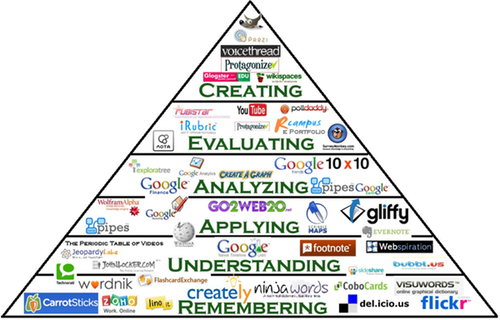
\includegraphics[width=0.85\textwidth]{Fig1.png}
 \caption{Pirámide de la Taxonomía Digital de Bloom.}
 \label{fig01}
 \source{\cite{penny_blooms_2015}}
\end{figure}

\subsection{Modelo de Maslow - Gerstein}\label{sec-modelo}
El modelo de Maslow o Jerarquía de necesidades de Maslow fue explicado por \textcite{gerstein_addressing_2014} desde la integración de la tecnología para satisfacer las necesidades del alumnado. Gerstein indica que trasladar este modelo a la educación es una forma ideal de evaluar planes curriculares, cursos y programas educativos. Conocer las necesidades del alumnado y preguntarse si estas necesidades se satisfacen en la escuela o en el aula, permite al profesorado integrar las TIC con previsión y con la intención de alcanzar objetivos específicos al mismo tiempo que orienta y potencia el aprendizaje del alumnado. En la \Cref{fig02} se muestra algunas de las estrategias de integración de tecnología que se puede utilizar para abordar los diferentes niveles de las necesidades de Maslow. 

\begin{figure}[h!]
 \centering
 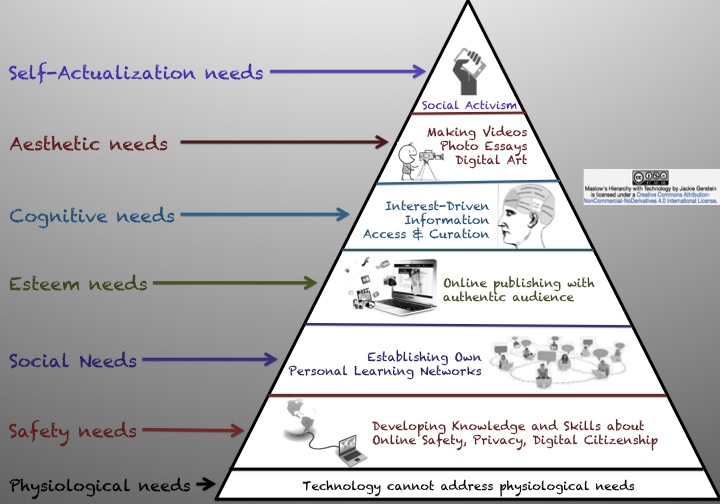
\includegraphics[width=0.85\textwidth]{Fig2.png}
 \caption{Pirámide de Maslow para la integración de las TIC.}
 \label{fig02}
 \source{\cite{gerstein_addressing_2014}}
\end{figure}

\textcite{gerstein_addressing_2014} explica los niveles que aparecen en la pirámide del siguiente modo:

\begin{enumerate}
    \item Necesidades biológicas y fisiológicas: aire, comida, bebida, refugio, sueño… en este caso, la tecnología no puede cubrirlas.
    \item Necesidad de seguridad: seguridad, orden, ley, estabilidad, protección… la tecnología y el uso de Internet ofrece beneficios y riesgos, y es importante que el profesorado sea consciente de los riesgos y de las medidas que puede tomar para minimizarlos. Actualmente, la seguridad gira en torno a la seguridad en línea, la ciudadanía digital, la privacidad y la prevención del ciberacoso. Se debe enseñarlo y reforzarlo continuamente para estudiantes de todas las edades. 
    \item Necesidades sociales: pertenencia, amor, familia, relaciones, afecto… Internet permite conectar con personas de todo el mundo que son afines a nosotros. Los docentes desarrollan estrategias para ayudar a su alumnado en su aprendizaje, les proporciona tiempo, recursos e incluso genera espacios de aprendizaje basados en redes o comunidades donde los alumnos pueden aumentar sus oportunidades de adquirir un sentido pertenencia y satisfacer sus necesidades sociales dentro de una comunidad. 
    \item Necesidad de estima: autoestima, logros, dominio, independencia, estatus, prestigio, responsabilidad, dominio…. Las personas necesitan sentirse valoradas y que contribuyen con la comunidad o con el mundo. En este caso, la creación tiene un gran potencial para aumentar la propia autoestima, y la tecnología proporciona las herramientas y medios para que los alumnos creen sus propios productos en lugar de ser meros consumidores (crear blogs, vídeos, música, videojuegos etc.). La tecnología no solo les permite crear, también les brinda la oportunidad de difundir, publicar y compartir sus creaciones con usuarios afines a través de plataformas de redes sociales.
    \item Necesidades cognitivas: conocimiento, significado. En este caso, se plantea cómo ayudar a los alumnos a satisfacer sus necesidades cognitivas. El profesorado ya no posee todo el conocimiento, pues Web 2.0 e Internet contienen multitud de recursos (audios, vídeos, investigaciones, manuales…) para ampliar los conocimientos y satisfacer esta necesidad. Para ello, Internet debe ser accesible y estar disponible para los estudiantes en el contexto escolar, sin limitarlos a usar el libro de texto, incluso permitirles reflexionar, crear y compartir contenido a través de las tecnologías (Blogs, wikis, radio educativa…). De esta forma, el profesor guía y orienta el proceso de aprendizaje. Así, los profesores pueden proporcionar a los alumnos temas y objetivos de aprendizaje deseables, y luego darles la libertad de buscar y compartir sus propios recursos sobre esos temas.
    \item Necesidades estéticas: apreciación y búsqueda de la belleza, el equilibrio, la forma… La tecnología ha ofrecido nuevas formas de participar y satisfacer las necesidades estéticas al impulsar la colaboración, publicación y difusión de arte u otras actividades creativas. La proliferación de las tecnologías y aplicaciones de la Web 2.0 promueve una corriente cultural amplia basada en la producción de manifestaciones artísticas: composición musical, danza, diseño y artes visuales (poesía, bailar, videojuegos, películas, cortos, libros, dibujos animados etc.). El profesorado puede aprovechar las habilidades e intereses de los alumnos para ayudarles a aprender sobre las áreas curriculares.
    \item Necesidades de autorrealización: darse cuenta del potencial personal, autorrealización, búsqueda del crecimiento personal y experiencias máximas. En este caso, se relaciona con la capacidad de aplicar lo que los estudiantes han aprendido y poder “retribuir” y participar en la mejora de la comunidad. Los foros en línea o las redes sociales tienen el potencial de ayudar a los estudiantes a involucrarse en causas sociales (servicio comunitario o voluntariado) y en el activismo social. Los profesores pueden utilizar el potencial y las habilidades de las redes sociales y el deseo de los estudiantes para promover el aprendizaje significativo y comprometido. Esto, a su vez, ayuda a preparar el escenario para que los alumnos desarrollen sentimientos de autorrealización.
\end{enumerate}

\section{De la enseñanza basada en TIC a la enseñanza virtual}\label{sec-organizacao}
La situación de confinamiento derivada por la pandemia causada por la Covid-19 a partir de marzo de 2020 alteró todos los ámbitos de nuestra sociedad y afectó gravemente a los sistemas educativos. Los cierres de instituciones educativas a los que obligó el confinamiento domiciliario obligatorio en muchas regiones del mundo provocaron cambios profundos en los modelos didácticos que tuvieron que implantarse de manera acelerada. Esto ocurrió en todos los niveles educativos. Los cambios en los modelos de enseñanza han tenido repercusiones que aún estamos investigando. La enseñanza virtual, que era residual o experimental, al estallar la pandemia se ha ido normalizando en la mayoría de las instituciones, acompañando las prácticas tradicionales de enseñanza presencial o sustituyéndola en bastantes casos \cite{fernandez_cruz_evaluation_2020}.

El nuevo paradigma de enseñanza que se abre nos obliga a estudiar los aspectos novedosos que afectan a la relación didáctica y, especialmente, los factores neurodidácticos que determinan el afrontamiento que realiza el estudiante de las nuevas metodologías de enseñanza y su repercusión en la persistencia, el éxito y el mejor aprovechamiento académico de los estudios. En este texto avanzamos en el estudio de los factores neurodidácticos de la enseñanza virtual desde varias ópticas.

La enseñanza virtual se desarrolla total o parcialmente a través de Internet y tanto las plataformas basadas en web, usadas preferentemente en computadoras de sobremesa o portátiles, como las aplicaciones móviles listas para teléfonos inteligentes, la hacen posible \cite{ko_teaching_2017}. A pesar de que la enseñanza virtual está presente en tres modelos formativos bien descritos por los expertos en la literatura, \textit{e-learning}, \textit{b-learning} y \textit{m-learning} \cite{bonk_moocs_2015,salinas_tic_2015,verdun_educacion_2016}, lo cierto es que el cierre universitario restringió la virtualidad de la nueva enseñanza a tan sólo dos de ellos, \textit{e-learning} y \textit{m-learning}, quedando el segundo restringido, de manera muy minoritaria, a algunas situaciones excepcionales de enseñanza. Ha sido el modelo que conocemos como \textit{e-learning} (\textit{electronic learning}) también denominado formación \textit{online}, educación a distancia o teleformación, en el que los procesos formativos se desarrollan en contextos exclusivamente virtuales, el que se ha impuesto durante los meses de confinamiento. No se trata más que de una forma de educación a distancia en la que los estudiantes y el profesor están separados en tiempo y espacio y los procesos de enseñanza y de aprendizaje se desarrollan de forma dinámica y flexible mediante el uso de las TIC \cite{garcia-marcos_autorregulacion_2020,gros_salvat_evolucion_2018}.

La práctica de la educación virtual es compleja y debe tener en cuenta las conexiones del proceso de enseñanza con el entramado de los factores que le dan sentido \cite{barbera_gregori_incognita_2001,telleria_educacion_2004}; el tipo de institución; la organización que la ofrece; qué clase de formación pretende; el marco de referencia del sistema educativo en el que se encuentra; los estudiantes que la solicitan; sus características e intereses; el rol del docente o profesor; el tipo de materiales de que se dispone; el currículo y la naturaleza propia del contenido objeto de aprendizaje; la concepción de evaluación y la disponibilidad de los recursos tecnológicos para lograr la comunicación-interacción de acuerdo al modelo pedagógico adoptado.

De acuerdo a lo anterior, los factores que inciden en la enseñanza virtual en el nivel de Educación Superior se configuran bajo tres ámbitos fundamentales:

\begin{enumerate}[label=\alph*.]
    \item Institución. Desde el punto de vista técnico, las instituciones deben virtualizar los espacios tradicionales para disponer de “aulas virtuales” que apoyen o sustituyan tecnológicamente las actividades académicas \cite{peterman_elements_2000}. Las herramientas de la institución (\textit{hardwares}, plataformas de \textit{software} etc.), las políticas, pautas o estándares que rigen los contenidos, los servicios y el apoyo de mantenimiento y formación que ofrecen, son factores que determinan la docencia virtual \cite{ko_teaching_2017}. Expertos como \textcite{clarke_corporate_2001} indican que la banda ancha, la presencia de ordenadores en las casas y los estándares tecnológicos mejorados, también son elementos que configuran la infraestructura tecnológica.
    \item Profesorado. El docente necesita comprender el nuevo espacio asincrónico y expandido de enseñanza y debe estar capacitado, interesado y disponer de los recursos necesarios para desarrollar la docencia virtual \cite{fernandez_cruz_formacion_2015}. De acuerdo con los Estándares de Competencia TIC para Docentes de la \textcite[p. 2]{unesco_estandares_2008}, el profesorado es el responsable de diseñar y generar oportunidades de aprendizaje. Por ello, en esta modalidad de enseñanza, el perfil docente debe contar con las competencias digitales necesarias para elaborar material de apoyo y recursos tecnológicos, diseñar materiales hipermedia y multimedia, utilizar \textit{software} y recursos informáticos para complementar la enseñanza, ser un guía en los procesos de aprendizaje, valorar los avances académicos de los estudiantes, coordinar grupos de aprendizaje colaborativo, motivar y propiciar la participación, facilitar la comunicación y la interacción, así como manejar adecuadamente los recursos y herramientas tecnológicas \cite{peterman_elements_2000,unesco_estandares_2008,tagliapietra_campus_2017}. Pues tal y como lo indica \textcite[p. 18]{coll_psicologieducacion_2004}, “el impacto de las TIC sobre las prácticas educativas no depende tanto de la naturaleza y las características de las tecnologías concretas que se utilizan, como del uso pedagógico que se hace de ellas”.
    \item Estudiantes. El rol del estudiante es determinante en el aprendizaje \textit{online}, ya que debe tener adquiridas las competencias digitales necesarias para garantizar su desenvolvimiento en el proceso de formación \cite{esteve_mon_nuevo_2011}. En este sentido, todas las áreas que configuran la competencia digital incluyen un conjunto de habilidades necesarias para interactuar de forma efectiva en el espacio virtual. Estas competencias poseen diversos grados; el nivel básico está relacionado con el uso y manejo de herramientas informáticas, la búsqueda, tratamiento y difusión de la información, mientras que el nivel avanzado, dependiendo del área académica, va más allá del dominio de \textit{softwares} específicos, pues requiere de habilidades cognitivas, motoras, sociológicas y emocionales para desenvolverse efectivamente en ambientes digitales \cite{valerio_urena_competencias_2012,fernandez_marquez_formacion_2017}. Por otro lado, los estudiantes aprecian más la flexibilidad del entorno virtual, así como la eliminación de los límites marcados por el tiempo, el espacio y la distancia de la educación presencial \cite{peterman_elements_2000}. Sin embargo, este tipo de aprendizaje virtual requiere una alta capacidad de autorregulación del aprendizaje para alcanzar los resultados deseados, lo que implica, una adecuada gestión y planificación del tiempo de estudio \cite{vohs_handbook_2016,van_laer_search_2017,garcia-marcos_autorregulacion_2020}.
\end{enumerate}

\section{Conclusiones}\label{sec-organizacao-latex}
A partir de la revisión realizada podemos asegurar -- lo hacemos en la línea de lo defendido por \textcite{fernandez_cruz_neuropedagogi_2022} --, que para que los docentes enseñen tal y como hoy les exige la sociedad y les compete a partir de los avances que está registrando la neurociencia,  deben estar en disposición de planificar  ambientes de aprendizaje óptimos que integren las tecnologías emergentes, que usen la enseñanza virtual, y que combinen todo ello con recursos de estímulo sensorial, perceptivo y atencional para lograr el desarrollo integral y el uso de metodologías personalizadas y participativas.

El reto de la ampliación de la educación básica y obligatoria a toda la ciudadanía y en todas las regiones del mundo obliga a replantearse, como aquí lo hemos hecho, el currículo formativo de los docentes para hacerlo coherente con el escenario social de la diversidad y articularlo en el aprendizaje de metodologías y prácticas pedagógicas innovadoras y de potenciación de las habilidades y capacidades únicas de cada alumno, de sus posibilidades de expresión y comunicación, así como de sus necesidades de interacción social. 

Este replanteamiento curricular sobre la formación inicial docente se fundamenta desde la responsabilidad que asume el profesor en el éxito o el fracaso educativo. Por lo tanto, para evitar prácticas educativas que no respondan a las exigencias curriculares y sociales actuales, se debe aunar y orientar los esfuerzos para que los elementos curriculares permitan, a los futuros docentes, entender cómo se produce el aprendizaje de forma fisiológica; potencien el dominio de los conocimientos que deben enseñar; cubran las deficiencias didácticas y, contribuyan a la adopción de un modelo pedagógico tecnológico, que a su vez, repercuta en el uso eficiente e innovador de los recursos digitales.

Por ello, los docentes necesitan adquirir un conocimiento sólido y estructurado que les permita, de forma natural, desarrollar prácticas didácticas más eficientes que induzcan al aprendizaje significativo y al desarrollo cerebral y psicodinámico, así como analizar y adaptar las herramientas digitales al contexto, al contenido y al objetivo de aprendizaje y, por ende, al contexto educativo y/o al proceso de enseñanza-aprendizaje.

Finalmente, en este contexto y teniendo en cuenta la realidad social, se concluye afirmando que es indiscutible la importancia de la neurodidáctica para diseñar la intervención educativa teniendo en cuenta cómo se produce el aprendizaje en el cerebro, así como de una cultura tecnológica que asuma modelos pedagógicos tecnológicos para integrar eficazmente las TIC en la práctica educativa. En definitiva, la formación inicial de los docentes se debe asentar sobre las bases de la neurodidáctica y los modelos pedagógicos tecnológicos de la acción formativa para promover un cambio en el paradigma educativo centrado en el estudiante, en el que se diseñen intencionada y estratégicamente las acciones didácticas, indistintamente del contexto presencial o virtual.


\printbibliography\label{sec-bib}
% if the text is not in Portuguese, it might be necessary to use the code below instead to print the correct ABNT abbreviations [s.n.], [s.l.]
%\begin{portuguese}
%\printbibliography[title={Bibliography}]
%\end{portuguese}

\end{document}

